\documentclass[journal]{IEEEtran}
% IEEE Journal of Oceanic Engineering 鈥?full draft v2
% Compile: pdflatex main.tex (twice)

\usepackage{amsmath,amssymb}
\usepackage{graphicx}
\usepackage{booktabs}
\usepackage{multirow}
\usepackage{url}
\usepackage{url}
\usepackage[colorlinks=true,linkcolor=black,citecolor=black,urlcolor=blue]{hyperref}

\newcommand{\pp}{\,\text{pp}}
\newcommand{\best}[1]{\textbf{#1}}
\newcommand{\eq}[1]{Eq.~(#1)}

\begin{document}

\title{Honest Evaluation of Underwater Acoustic Target Recognition:\\
Decomposing, Predicting, and Reducing Benchmark Variance}

\author{\IEEEauthorblockN{Zihao~Gong,~Debiao~Li,~Juncheng~Liu,~Junrui~Guo,~Qi~Gong,~and~Yongqiang~Xie}
\IEEEauthorblockA{Z.~Gong, D.~Li, and Y.~Xie: School of Mechanical Engineering,
Xidian University, Xi'an 710071, China (andy.zihao.gong@gmail.com;
lidehu64@gmail.com; yqxie@xidian.edu.cn)}
\IEEEauthorblockA{J.~Liu: School of Information and Communication Engineering,
Guilin University of Electronic Technology, Guilin 541004, China (3409674230@qq.com)}
\IEEEauthorblockA{J.~Guo: School of Mechano-Electronic Engineering, Xidian University,
Xi'an 710071, China (guojunrui@stu.xidian.edu.cn)}
\IEEEauthorblockA{Q.~Gong: Petroleum and Natural Gas Engineering,
Southwest Petroleum University, Chengdu 610500, China (kungclive.8804@gmail.com)}
\thanks{Z.~Gong and D.~Li contributed equally to this work. Corresponding author:
Yongqiang~Xie (e-mail: yqxie@xidian.edu.cn).}%
\thanks{All frozen splits, allocation code, per-clip predictions, and the required-$N$
calculator are released for replication.}}

\markboth{IEEE Journal of Oceanic Engineering --- Draft}%
{Gong \MakeLowercase{\textit{et al.}}: Honest Evaluation of Underwater Acoustic Target Recognition}

\maketitle

\begin{abstract}
Identity-disjoint evaluation is now the recommended convention in underwater acoustic target
recognition (UATR), but its statistical cost has never been quantified. On OceanShip (12 classes),
the vessel-disjoint accuracy of an identical model varies by $\pm$5.0\,pp across 25 independent
draws---twelve times the clip-level noise---while the nominal clip-vs-honest gap is
5.1\,pp on OceanShip but 30.4\,pp on DeepShip under identical code and recipe. We show that this
draw-to-draw variance is dominated (89\% in-sample; 59\% out-of-sample under leave-one-draw-out)
by the class composition of the test set, computable from metadata before any training; that a
first-order predictor calibrated on this decomposition correctly estimated the observed spread of
five allocation schemes across three model families; and that a class-wise clip-mass stratified
allocation collapses the variance to the lowest level observed across the tested allocations (4.69
to 1.24\,pp; variance
ratio 14.4, exact permutation $p=0.004$), reducing the draws needed to resolve a 2\,pp improvement
from about 100 to 8 per system (10--13 to 3--7 when comparisons are fully paired). Consistently
across models, the remedy shows no benefit on DeepShip, where composition-induced variability is small relative to the observed draw variability. The
low absolute accuracy of honest evaluation is not a pipeline defect: five tested
interventions---capacity growth, post-hoc prior adjustment, selective prediction, frozen
pretraining, and full fine-tuning---fail to decode the nine-class tail, and a training-mass
diagnostic shows recall tracks clip identity mass; the tail's three-tier structure is itself
predicted from metadata. Frozen splits, allocation code, and a
required-$N$ calculator are released.
\end{abstract}

\begin{IEEEkeywords}
Underwater acoustic target recognition, vessel-disjoint evaluation, benchmark variance,
group-stratified allocation, data leakage.
\end{IEEEkeywords}

\section{Introduction}
\IEEEPARstart{R}{ecent} guidance in underwater acoustic target recognition (UATR) has converged on
a simple methodological prescription: do not evaluate with clip-level random splits. Adjacent clips
of one recording share background noise and propagation conditions \cite{review2026}, so a random
clip split places near-duplicates on both sides of the train/test boundary, and the resulting
accuracy measures retrieval of a known recording as much as recognition of a ship type. The 2026
survey of the field lists the accuracy gaps between random, temporal, and recording-level splits
explicitly \cite{review2026}; UniqueShip \cite{uniqueship2026} re-quantifies the inflation at
10--48\pp{} across corpora and proposes identity-grouped re-splits; and recent systems work adopts
recording-level splits with significance testing \cite{boosting2026}. Within the general
machine-learning literature, leakage taxonomies \cite{kapoor2023} and variance accounting
\cite{bouthillier2021} provide the conceptual vocabulary.

This paper starts from the observation that the guidance leaves out: \emph{honest evaluation has a
noise floor, and, to our knowledge, no one has measured it.} When the unit of allocation is the vessel or the
recording, each random draw changes which ships---and therefore which classes---land in the test
set. On OceanShip, a public benchmark with vessel identities, the test accuracy of an
identical model under identical training varies by $\pm5.0$\pp{} from one vessel-disjoint draw to
the next (25 independent draws), while the clip-random baseline varies by $\pm0.4$\pp. The honest protocol is therefore
simultaneously more meaningful and twelve times noisier; a paper reporting a single honest-protocol
number is reporting an estimate whose uncertainty exceeds most published method improvements. And
because the noise is driven by \emph{which classes} the draw samples, it is not statistical
background: it is a property the benchmark's own metadata determines and exposes.

We make four contributions.
\begin{enumerate}
\item \textbf{A variance decomposition of honest evaluation}
      (Sec.~\ref{sec:variance}). We split the draw-to-draw variance into a \emph{composition}
      component (which classes the draw places in the test set; pure metadata, computable before
      training) and a residual component (initialization, optimization, and any remaining
      draw-level effects). On OceanShip the
      composition component explains 89\% of the vessel-disjoint variance over 25 independent
      draws (permutation $p=0.0006$), 54\% at the intermediate
      recording level, and 0\% at the clip level: the more honest the protocol, the more the score
      is determined by metadata ($0\%\!\to\!54\%\!\to\!89\%$).
\item \textbf{A validated, calibration-based predictor} (Sec.~\ref{sec:predictor}). Fed with one pooled
      per-class recall table (measured once from trained models---scoring any candidate allocation
      requires no retraining) and the splits' class composition, the model predicted the observed
      draw spread of five independent allocation schemes across three model families, and correctly
      predicted the \emph{absence} of fixable variance on DeepShip
      (Sec.~\ref{sec:control}).
\item \textbf{A remedy with measured variance reduction} (Sec.~\ref{sec:remedy}). A class-wise
      clip-mass stratified allocation---assigning whole vessels until each class has contributed
      its quota of \emph{clips}---collapses the honest-protocol variance to the lowest level
      observed across the tested allocations ($4.69\pp \to 1.24\pp$; variance ratio 14.4, exact
      permutation $p=0.004$), generalizes across
      a linear probe and a $4\times$ wider CNN, and reduces the draws needed to resolve a 2\pp{}
      improvement from about 100 independent draws to 8---and paired two-model comparisons need
      3--7 draws rather than 10--13. A naive stratification balancing \emph{vessel counts} instead of
      clip masses fails exactly as the decomposition predicts.
\item \textbf{The limits of tested remedies} (Sec.~\ref{sec:limits}). The low absolute accuracy of
      honest evaluation is not a pipeline defect: five tested interventions---capacity growth,
      post-hoc prior adjustment, selective prediction, frozen pretrained encoders, and full
      fine-tuning---fail to decode the nine-class tail, a training-mass diagnostic explains part
      of the pattern, and the three-tier structure
      (learnable, partially rescuable, intervention-resistant) is predictable from metadata.
\end{enumerate}

Throughout, we separate two quantities that the leakage literature tends to conflate: the
\emph{existence} of leaky information (provable from metadata: on OceanShip, predicting a test
clip's label from the majority label of its training vessel reaches 99.4\%) and its
\emph{acoustic exploitability} (a nearest-neighbour probe on the features reaches only 25.5\%, with
same-recording neighbours at 5.7\% versus a 0.03\% chance rate). On DeepShip, where recordings are
tiled into contiguous 5\,s windows, a single scalar---the source-file duration, one value per
recording---retrieves 78.2\% of clip-random accuracy without listening to the audio. Existence
without exploitability, and exploitability without existence, are different failure modes with
different remedies; we measure both (Sec.~\ref{sec:leak}).

\section{Related Work}
\subsection{Leakage in ML-Based Science}
Kapoor and Narayanan \cite{kapoor2023} enumerate leakage types across disciplines; duplicate-adjacent
and non-independent train/test samples (their L1.4/L3.2) are the UATR case. Recent work formalizes
the distinction we exploit: metadata predictability of an output (MPDS) is logically independent of
the output's dependence on the underlying evidence \cite{mpds2026}. In audio specifically,
mel-similarity audits have surfaced tens of millions of overlapping pairs across popular datasets,
and UniqueShip \cite{uniqueship2026} re-quantifies leakage for acoustic ship classification,
reporting 10--48\pp{} inflation under random splits and proposing identity-grouped re-splits. Our
work is complementary: we take identity grouping as given and ask what it does to the
\emph{reliability} of the resulting evaluation.

\subsection{Evaluation Noise and Variance}
Bouthillier et al.\ \cite{bouthillier2021} showed that data-sampling variance dominates
initialization variance in general ML benchmarks; Gillick and Cox \cite{gillick1989} established
matched-pairs significance testing for speech evaluation---the same paired-across-draws design we
use throughout; recent UATR guidance discusses grouped evaluation at the recording level
\cite{review2026}.
None of these quantify
\emph{which} component of group-disjoint variance is metadata-predictable, nor the number of draws
required for a given effect size---the two numbers a practitioner actually needs.

\subsection{Group-Stratified Splitting}
Stratified group $k$-fold \cite{sklearn} balances class margins across folds while keeping groups
intact, and count- or margin-balanced group variants are standard tooling. We do not claim a new
algorithm: our clip-mass allocator is a quota variant of the same idea, distinguished by (i)
balancing the per-class \emph{clip mass} of vessels rather than their counts---a distinction the
data proves matters (Sec.~\ref{sec:remedy})---and (ii) being validated by a pre-specified,
decomposable variance model rather than offered as a heuristic; none of the standard variants
ships with a variance model that says when balancing matters at all.

\subsection{UATR Benchmarks and Systems}
DeepShip \cite{deepship} and ShipsEar \cite{shipsear} tile or excerpt recordings into labeled
clips; OceanShip \cite{oceanship} adds vessel identities (MMSI) and AIS metadata. Systems work
adopts recording-level splits with statistical checks \cite{boosting2026}; transfer-learning
studies report that embedding spaces are dominated by recording-specific factors
\cite{hummel2026}; open-set recognition, contrastive generalization \cite{aa2025contrastive},
adversarial individual-vessel generalization \cite{fang2025}, and physics-informed architectures
\cite{mmipfnn2026} target the accuracy race under various protocols.
Our audit explains a cross-cutting observation in this literature: under honest evaluation,
12-class OceanShip collapses to three effective classes while 4-class DeepShip does not
(Sec.~\ref{sec:limits})---a consequence of class granularity that no accuracy number reveals by
itself.

\section{Data, Protocols, and Models}
\label{sec:setup}

\subsection{Corpora}
\textbf{OceanShip} \cite{oceanship} is the primary benchmark: 53{,}770 clips from 10{,}168
hydrophone recordings of 892 vessels (MMSI), labeled by AIS ship type, 5\,s clips at 32\,kHz. We
evaluate the 12 classes with at least 3 vessels; the 3 rare classes (Diving ship, Military ship,
Spare; 139 clips) are excluded from all splits, matching how the frozen baseline splits define the
task. Recordings are arbitrary-length excerpts of a hydrophone stream: the median recording
contains 3 clips (maximum 210), and the trailing index of a clip id is \emph{not} a stream
position---two clips of one recording are arbitrary moments, not adjacent windows.
\textbf{DeepShip} \cite{deepship} (47\,h, 609 recordings, 4 classes) is the structural opposite:
recordings are tiled by back-to-back 5\,s windows (median 51 clips per recording;
$\text{clips}\times5\,\text{s}/\text{duration}\approx0.99$; the clip index equals stream position
for 609/609 recordings). \textbf{ShipsEar} \cite{shipsear} (2{,}223 clips, 11 classes) is used only
for leakage statistics. Table~\ref{tab:corpora} contrasts the corpora; this slicing policy, as we
show in Sec.~\ref{sec:leak}, is the hidden variable that makes ``random split'' incomparable
across papers.

\begin{table}[!t]
\caption{Corpora and Slicing Policy}
\label{tab:corpora}
\centering
\footnotesize\setlength{\tabcolsep}{3.2pt}
\begin{tabular}{lcc}
\toprule
 & OceanShip & DeepShip \\
\midrule
recordings                 & 10{,}168 & 609 \\
clips                      & 53{,}770 & 33{,}770 \\
classes (evaluated)        & 12 (of 15) & 4 \\
clips / recording (median) & 3        & 51 \\
tiling ratio (clips$\times$5\,s / duration) & n/a & 0.994 \\
clip index = stream position & no & 609/609 \\
test clips with adjacent training clip & n/a (index is not stream position) & 89.6\% \\
acoustic 1-NN nearest training clip from same recording & 5.7\% & 66.8\% \\
clip $-$ honest gap        & $+5.1$\pp & $+30.4$\pp \\
\bottomrule
\end{tabular}
\end{table}

\subsection{Split Protocols}
For OceanShip we use three allocation units: \textbf{clip random} (clips assigned independently;
the leaky convention), \textbf{recording random} (recordings intact; ships still cross sets), and
\textbf{vessel disjoint} (no MMSI on both sides; the honest protocol). For DeepShip the analogues
are clip random, recording random, and temporal. All splits are frozen files generated by a
deterministic SHA-256-seeded procedure (independent of Python's salted \texttt{hash}), verified for
zero group intersection at write time and re-verified by the training runner at read time; split
draws and network initialization use separate seeds. Protocol names are never trusted: the runner
rejects a split file that does not contain the requested (protocol, seed) pair, and a stalled
schedule aborts the run. Fig.~\ref{fig:schematic} shows what each policy lets cross the boundary.

\begin{figure}[!t]
\centering
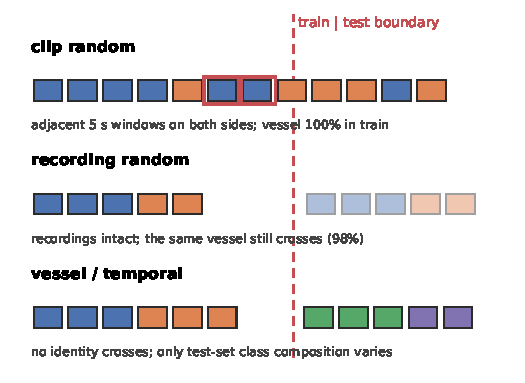
\includegraphics[width=\columnwidth]{figures/fig_schematic.pdf}
\caption{What crosses the split boundary under each slicing policy (one row of squares = the clips
of one or two vessels). Clip random puts adjacent 5\,s windows of the \emph{same audio event} on
both sides and the vessel's identity in the training set; recording random keeps recordings intact
but still lets $98\%$ of vessels cross; vessel/temporal isolation crosses nothing---and thereby
turns test-set class composition into a random variable, the subject of
Sec.~\ref{sec:variance}.}
\label{fig:schematic}
\end{figure}

\subsection{Models and Training Recipe}
The reference model is \texttt{cnn\_small} (136{,}692 parameters) trained on log-mel spectrograms
(128 mels $\times$ 313 frames) for 24 epochs with AdamW (lr $3\times10^{-3}$, 3 warm-up epochs,
cosine decay, batch 64). The recipe was fixed by a wiring check (the model memorizes 512 clips to
99.2\% in 200 epochs; a ResNet-18 memorizes the full training set to 0.9999) and never changed
across any table in this paper; every run logs the final learning rate, and a guard aborts any run
whose schedule never stepped---two silent failures we encountered and eliminated early. Model
families for the remedy experiments: \texttt{logreg} (multinomial logistic regression on the
flattened spectrogram; 480{,}780 parameters) and \texttt{cnn\_wide} (542{,}940 parameters). Each
run stores per-clip predictions with recording/vessel identity, enabling recording-level bootstrap
and per-class decomposition. Table~\ref{tab:recipe} lists the full recipe; it is intentionally
modest, because every claim in this paper is about the evaluation protocol, not about pushing
accuracy---and the interventions in Sec.~\ref{sec:limits} bound how much model choice could change
our conclusions.

\begin{table}[!t]
\caption{Training Recipe (identical for every run in Tables II--VI)}
\label{tab:recipe}
\centering
\footnotesize\setlength{\tabcolsep}{3.2pt}
\begin{tabular}{ll}
\toprule
input & log-mel $128\times313$, per-clip standardized \\
optimizer & AdamW, batch 64, weight decay $10^{-4}$ \\
schedule & cosine, 3 warm-up epochs, peak lr $3\times10^{-3}$ \\
epochs & 24 (200 for the 512-clip wiring check) \\
guards & per-epoch lr log; abort if schedule never steps \\
model selection & final epoch (val used only for fine-tuned AST) \\
logging & per-clip predictions with recording/vessel id \\
seeds & split draw and initialization decoupled \\
\bottomrule
\end{tabular}
\end{table}

\subsection{Pre-Registration Protocol}
Every comparison in this paper was registered before its runs: the verdict thresholds (e.g., the
remedy succeeds iff the SD ratio is $\le0.6$; the fine-tuning door opens iff tail top-2
$\ge0.30$), the control predictions, and the identity-floor prediction for the $<5$-vessel classes
were written down before the corresponding GPU jobs. Where a prediction failed---our first remedy
candidate, weighting by vessel \emph{counts}, was rejected by a zero-cost dose--response check
before any training---we report it (Sec.~\ref{sec:remedy}). We consider this discipline part of
the contribution: the audit's claims are exactly as strong as their pre-registration.

\section{Leakage: Existence Versus Exploitability}
\label{sec:leak}

\subsection{Metadata Ceilings}
The metadata ceiling---predicting each test clip's label by the majority training label of its
vessel, using no audio---is 99.44\% on OceanShip clip-random (99.5\% coverage) and 98.16\% at the
recording level; on DeepShip clip-random the recording ceiling is 99.82\%. These numbers quantify
\emph{existence}: what the allocation hands over. Labels themselves are clean---no OceanShip
recording is multi-labeled, and only 5 of 892 vessels are cross-class (1.1\% of clips)---so
identity lookup is a legitimate oracle, not label noise.

\subsection{Acoustic Exploitability}
Existence does not imply exploitability. On 16$\times$16 pooled log-mel descriptors, the 1-NN probe
finds a same-recording nearest training clip for only 5.7\% of OceanShip test clips---180$\times$
above the 0.03\% chance rate, so recording identity \emph{is} in the features---but weak and
diffuse; 1-NN label accuracy is 25.5\% against a 22.1\% constant baseline, and a ridge probe on the
256-D descriptor reaches 27.4\%. On DeepShip the picture inverts: 1-NN label accuracy is 83.2\%
(27.2\% constant), same-recording neighbours at 66.8\% (234$\times$ chance), and 36.8\% of them are
the immediately adjacent 5\,s window.

\subsection{One Scalar Is Enough---Where Recordings Are Tiled}
DeepShip's \texttt{src\_dur\_s} column is the \emph{source-file duration}, one value shared by
every 5\,s window cut from that file. It is therefore a recording fingerprint. A nearest-neighbour
classifier on this \emph{single scalar}---no audio, no training---reaches 78.2\% (five draws:
78.2--80.0\%) on clip random, compared with 83.2\% for a 256-D acoustic descriptor and 92.2\% for
the trained model. The ordering is the finding. Under recording-level splits the scalar collapses
to 34.6\% (recording random) and 21.8\% (temporal), at or below the constant baseline: what the
scalar buys is \emph{identity}, not ship type. On OceanShip the same scalar reaches only 9.3\%,
because clip duration is not a recording fingerprint there. Table~\ref{tab:leak} summarizes and
Fig.~\ref{fig:probe} shows the ladder: under clip random, a metadata scalar with no audio nearly
matches an acoustic descriptor and a trained CNN; under honest splits every identity-linked
advantage collapses toward chance, exposing what the leaky number was made of.

\begin{figure}[!t]
\centering
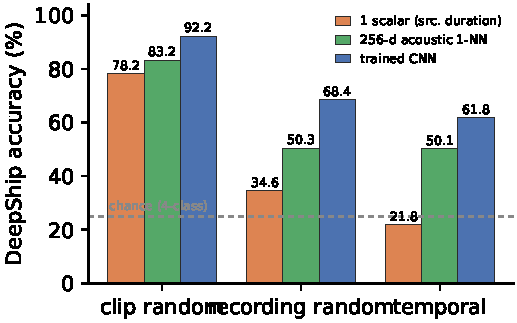
\includegraphics[width=\columnwidth]{figures/fig_probe.pdf}
\caption{The one-scalar probe on DeepShip (seed 0): accuracy of a single metadata scalar
(source-file duration 1-NN), a 256-d acoustic descriptor 1-NN, and the trained CNN under the
three slicing policies. The scalar's 78.2\% under clip random buys \emph{identity}, not ship
type---it collapses to near chance once recordings are isolated, while the acoustic probes lose
far less. Data from the released recording-structure audit.}
\label{fig:probe}
\end{figure}

\begin{table}[!t]
\caption{Leakage: Existence vs.\ Exploitability (seed-0 draws, no audio for ceilings/scalar)}
\label{tab:leak}
\centering
\footnotesize\setlength{\tabcolsep}{3.2pt}
\begin{tabular}{lcc}
\toprule
 & DeepShip & OceanShip \\
\midrule
metadata ceiling (vessel), clip random   & 97.5\% & 99.4\% \\
metadata ceiling (recording), clip random & 99.8\% & 90.8\% \\
1-NN label accuracy                      & 83.2\% & 25.5\% \\
\ \ (constant baseline)                 & (27.2\%) & (22.1\%) \\
1-NN shares the recording                & 66.8\% & 5.7\% \\
\ \ (chance rate)                       & (0.29\%) & (0.03\%) \\
adjacent-window neighbours               & 36.8\% & n/a$^{\dagger}$ \\
one-scalar (source duration) 1-NN        & 78.2\% & 9.3\% \\
trained model, clip random               & 92.2\% & 36.7\% \\
\bottomrule
\multicolumn{3}{l}{\footnotesize $^{\dagger}$OceanShip carries no stream position; the}\\
\multicolumn{3}{l}{\footnotesize absence itself is a slicing-policy fact.}
\end{tabular}
\end{table}

The official OceanShip split quantifies the stakes. In the benchmark authors' own configuration,
91.8\% of vessels and 19.8\% of recordings appear on both sides of the split; our clip-random
reconstruction reaches 99.6\% and 85.0\% of test recordings respectively (the 85.0/90.8/91.1\%
figures quoted in this paper use different units---by recording vs.\ by clip---and must be stated
when quoted). Against these baselines, the vessel-disjoint protocol is not a refinement but a
category change; everything in Secs.~\ref{sec:variance}--\ref{sec:control} is about making that
category change usable.

\section{The Anatomy of Honest-Evaluation Variance}
\label{sec:variance}

\subsection{The Same Protocol Name Is Not a Specification}
Table~\ref{tab:ladder} and Fig.~\ref{fig:ladder} give the ladder. On OceanShip, the same model and
recipe score $0.367$ under clip random and $0.316$ under vessel disjoint: the paired leak is
$+5.1$\pp{} (draw SD of the paired difference 4.5\pp, paired $t$ $p=0.064$)---at five draws the
leak itself sits at the edge of significance, which is the noise-floor point of this section, not
a weakness of the test. On DeepShip the same nominal comparison
spans $0.922 \to 0.618$: $30.4$\pp, and the true vessel-disjoint protocol---run with ten draws
after the temporal numbers were frozen---lands at $0.624\pm5.4$\pp, within $0.6$\pp{} of
temporal: two disjoint honest protocols agree with each other and sit $30$pp below the leaky
one. The reason is structural (Table~\ref{tab:corpora}): DeepShip's
clip-random test clips have an adjacent 5\,s window in the training set 89.6\% of the time---the
two clips are the \emph{same audio event}---whereas on OceanShip a test clip's nearest training
neighbour shares its recording only 5.7\% of the time. ``We used a random split'' is not a
comparable specification, and no dataset paper states how its recordings were cut into clips.
The DeepShip numbers also calibrate the pipeline against the literature: our honest-protocol
accuracy (0.618; pooled macro-F1 $0.61$ on the harder vessel-disjoint protocol) sits below the
best recording-level DeepShip figure we are aware of ($0.7226$ macro-F1 \cite{soti2026}), with a
far smaller model---as expected when moving to a strictly harder protocol; order-of-magnitude
agreement, not replication.

\begin{table*}[!t]
\caption{The Protocol Ladder (mean $\pm$ draw SD; log-mel, \texttt{cnn\_small})}
\label{tab:ladder}
\centering
\footnotesize\setlength{\tabcolsep}{6pt}
\begin{tabular}{lccc}
\toprule
Protocol & OceanShip & OceanShip & DeepShip \\
 & log-mel & log-mel spec & log-mel \\
\midrule
clip random      & $0.367\pm.004$ & $0.365\pm.004$ & $0.922\pm.006$ \\
recording random & $0.351\pm.013$ & $0.346\pm.013$ & $0.684\pm.029$ \\
honest (vessel/temporal) & $0.320\pm.050$ & $0.312\pm.048$ & $0.618\pm.009$ \\
vessel-disjoint (DeepShip, $n{=}10$) & & & $0.624\pm.054$ \\
\midrule
clip $-$ honest (paired) & $+5.1\pm4.5$\pp{} ($p{=}.064$) & $+5.3\pm4.6$\pp{} ($p{=}.063$) & $+30.4\pm0.8$\pp{} ($p{=}.002$) \\
\bottomrule
\end{tabular}
\vspace{2pt}

{\footnotesize A tag-aware recording-cluster bootstrap ($B{=}2000$) over all released draws
confirms the ladder and quantifies the allocator effect on OceanShip vessel-disjoint draw SD:
$5.0$\pp{} random ($n{=}25$), $4.9$ count-stratified, $2.6$ SGKF, $1.2$ clip-mass ($n{=}6$)—the
same ordering on \texttt{cnn\_wide} and \texttt{logreg}: the allocator a comparison inherits, not
the number of draws, decides the observed noise level. DeepShip vessel-disjoint: ten draws over 290 vessel
groups (48 AIS-unjoined recordings kept as singletons), every run verified at $0\%$ overlap of
recordings and \emph{known} identities (the 48 are guaranteed distinct recordings, not distinct
ships—see below); it lands $0.6$\pp{} from temporal ($t$95 $[0.585,0.663]$)---two disjoint honest
protocols, one number---and $30.8$\pp{} below clip random; paired over the three shared seeds the
clip$-$vessel leak is $+28.5\pm1.7$\pp{} ($p=0.001$). Singleton sensitivity: excluding those 48
recordings (ten draws) shifts the mean to $0.567$ (SD $4.4$\pp; $t$95 $[0.536,0.599]$), $5.7$\pp{}
below full-corpus (Welch $p=0.02$)---\emph{consistent with} residual identity leakage, though the
exclusion also changes the test composition (29\% explained, $p=0.54$); we report direction and
magnitude and disclose the singleton mass rather than claim a causal estimate. Pooled macro-F1:
$0.11\pm1.4$\pp{} (OceanShip vessel), $0.61\pm5.4$\pp{} (DeepShip vessel). Draw counts differ per
column: OceanShip clip/recording 5, vessel 25; DeepShip clip/recording/temporal 3, vessel 10.}
\end{table*}

\begin{figure}[!t]
\centering
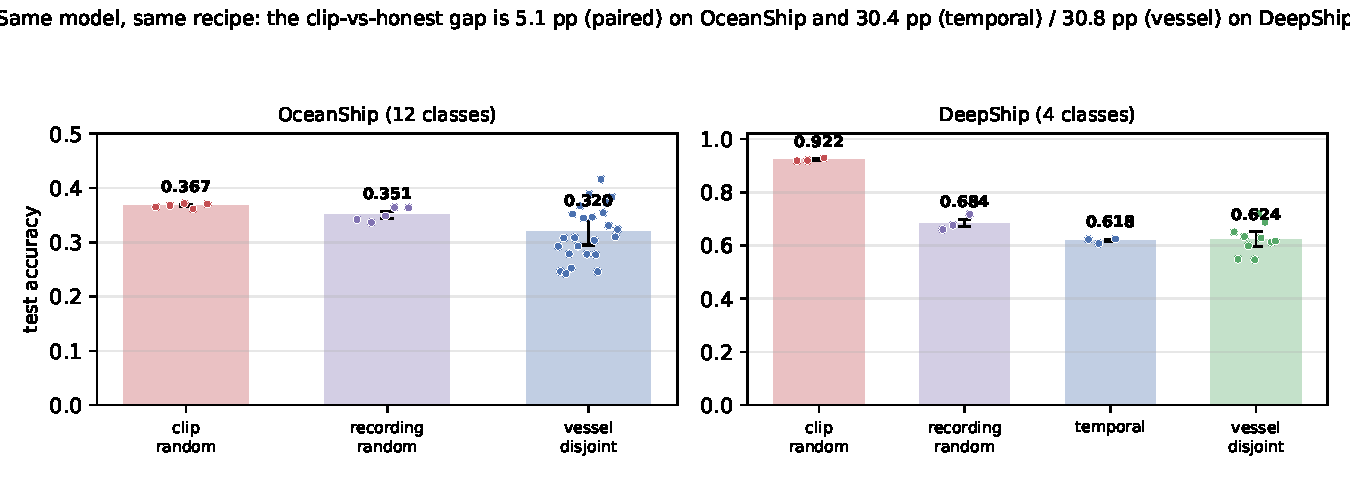
\includegraphics[width=0.84\columnwidth]{figures/fig_ladder.pdf}
\caption{The protocol ladder on both corpora; each dot is one independent draw, bars mark scheme
means ($\pm$SD/2). Same code, model, recipe; clip-vs-honest gap: 5.1\pp{} (paired) on OceanShip,
30.4 / 30.8\pp{} (temporal / vessel, $n{=}10$) on DeepShip; the honest draw spread dwarfs the
leaky protocol's.}
\label{fig:ladder}
\end{figure}

\subsection{Decomposing the Draw Variance}
Let the draws of a scheme partition vessels into train/validation/test. Each draw $d$ induces a
test-set class composition $n_d(c)$ (number of test clips of class $c$). Holding the model fixed,
\begin{equation}
\mathrm{acc}_d \;\approx\; \frac{1}{N_d}\sum_{c} n_d(c)\, r(c),
\label{eq:comp}
\end{equation}
where $r(c)$ is the per-class recall and $N_d=\sum_c n_d(c)$. We estimate $r(c)$ once, pooled over
the draws of the scheme, and predict each draw's accuracy from its composition alone;
Eq.~\eqref{eq:comp} would be exact if the per-class recalls were identical across draws; what it
ignores is draw-to-draw variation in the recalls themselves, not class interactions. The variance of
the predicted accuracies is the \emph{composition component}; the variance of the residuals
(observed minus predicted) is the \emph{residual} component---initialization and optimization
noise \emph{plus} any remaining draw-level effects (training-set composition, vessel difficulty). It is an empirical explained share, not an identified set of independent variance components, and
the estimator differs by row of Table~\ref{tab:decomp}. For the vessel row (25 draws $\ge$ 12
classes) the composition component is the least-squares projection of the observed accuracies onto
the composition shares: residuals are orthogonal to fitted values, so the covariance term vanishes
by construction (measured $2\,\mathrm{Cov}(C,E)<0.01$\pp$^2$) and the components add in quadrature,
$4.69^2+1.64^2=4.97^2$. For the clip and recording rows (5 draws, where OLS is underdetermined)
$r(c)$ is the clip-pooled per-class recall measured on the same draws. The clip row is trivially
additive ($\mathrm{Var}(C)=0$); the recording row is not---$2\,\mathrm{Cov}(C,E)=0.20$\pp$^2$---so
its 54\% is the variance ratio $\mathrm{Var}(C)/\mathrm{Var}(A)$, not an orthogonal share
(cross-terms are footnoted in Table~\ref{tab:decomp}). At
the clip level, where every draw places the same class masses in the test set, this residual is
bounded at $0.41$\pp, which plausibly reflects initialization and optimization; at the vessel
level the residual is larger ($1.65$\pp) and necessarily contains more than initialization alone.

Table~\ref{tab:decomp} gives the result on the reference model. The composition component explains
\textbf{89\%} of the vessel-disjoint variance over 25 independent draws (composition SD 4.69 of
4.97\pp; permutation $p=0.0006$), 54\% at the recording level,
and 0\% at the clip level, where the five draws place nearly identical class masses in the test
set. Two consequences follow. First, the honest protocol's noise is mostly \emph{metadata}: it can
be computed before training and removed by design. Second, Eq.~\eqref{eq:comp} is a falsifiable
predictor, which we test next---including in the direction of ``nothing to fix''
(Sec.~\ref{sec:control}).

\begin{table}[!t]
\caption{Variance Decomposition on OceanShip (\texttt{cnn\_small}, log-mel; clip/recording
5 draws, vessel 25 draws)}
\label{tab:decomp}
\centering
\footnotesize\setlength{\tabcolsep}{3.2pt}
\begin{tabular}{lcccc}
\toprule
Protocol & observed SD & composition SD & share & residual SD \\
 & (pp) & (pp) & (\%) & (pp) \\
\midrule
clip random      & 0.41 & 0.00 & 0  & 0.41 \\
recording random & 1.25 & 0.92 & 54 & 0.72 \\
vessel disjoint  & \best{4.97} & \best{4.69} & \best{89} & 1.65 \\
\bottomrule
\end{tabular}
\vspace{2pt}

{\footnotesize Composition SD: vessel row = least-squares projection (25 draws, $2\,\mathrm{Cov}(C,E)<0.01$\pp$^2$);
clip/recording rows = fixed pooled per-class recalls (5 draws; recording cross-term
$2\,\mathrm{Cov}(C,E)=0.20$\pp$^2$, so the components are not orthogonal there). The share is
$\mathrm{Var}(C)/\mathrm{Var}(A)$ throughout.}

\end{table}

\begin{figure}[!t]
\centering
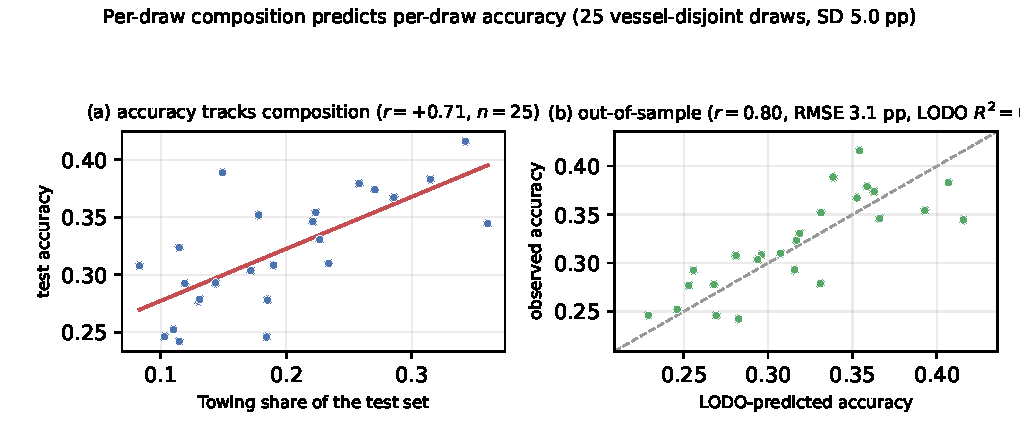
\includegraphics[width=0.94\columnwidth]{figures/fig_decomp.pdf}
\caption{Out-of-sample anatomy of the decomposition of Table~\ref{tab:decomp} (25 vessel-disjoint
draws). (a) Per-draw accuracy versus the draw's Towing clip-mass share (Pearson $r=+0.71$) with
the fitted relation: composition is the mechanism, visible draw by draw. (b) Leave-one-draw-out
predicted versus observed accuracy ($r=0.80$, RMSE $3.1$\pp): the composition model predicts
accuracies of draws it has never seen.}
\label{fig:decomp}
\end{figure}

\subsection{The Composition Model Predicts Real Experiments}
\label{sec:predictor}
Fig.~\ref{fig:pred} plots predicted versus observed draw SD for five independent allocation schemes
spanning three model families: clip-mass stratified allocation for
\texttt{cnn\_small}/\texttt{logreg}/\texttt{cnn\_wide}, count-stratified allocation, and
\texttt{StratifiedGroupKFold} \cite{sklearn}. All five lie on or near the identity line
($1.12\!\to\!1.24$, $0.70\!\to\!0.94$, $0.92\!\to\!1.36$, $4.85\!\to\!4.85$, $2.28\!\to\!2.60$\pp).
The predictor consumes the splits' class composition and one pooled per-class recall table; it
never sees the training outcomes of the schemes it predicts. Calibration and prediction are
disjoint by construction: the recall table is estimated on the reference scheme's own random
draws and frozen, and the schemes it scores were drawn \emph{after} that table was frozen
(Sec.~\ref{sec:threats}). The residual gap
(observed slightly above predicted) is consistent with the residual draw-level variability
quantified in Table~\ref{tab:decomp}. In Sec.~\ref{sec:control} the same model makes a \emph{null} prediction on
a second corpus---that there is nothing to fix---which is also confirmed.
Out-of-sample honesty, audited by leave-one-draw-out prediction on the 25-draw vessel pool:
fitting on 24 draws and predicting the held-out draw from its composition alone gives $r=0.80$
(permutation $p=0.0002$, RMSE $3.1$\pp) and LODO $R^2=0.59$ against the in-sample $0.89$: per-draw
accuracy is predictable for unseen draws at $\pm3$\pp, while the 89\% share is a population
statement; we report both to keep the in-sample optimism visible.

\begin{figure}[!t]
\centering
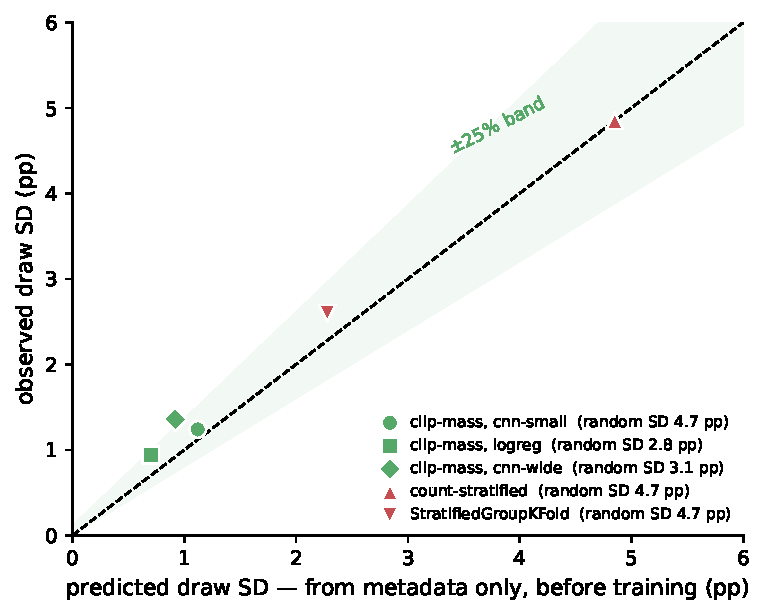
\includegraphics[width=0.82\columnwidth]{figures/fig_pred.pdf}
\caption{Predicted vs.\ observed draw-to-draw SD for five allocation schemes (three model
families); shaded band $\pm25\%$. The calibration-based model tracks the identity line without
seeing any training outcome of the schemes it predicts; the legend gives each scheme's
random-draw SD.}
\label{fig:pred}
\end{figure}

\section{A Metadata-Only Remedy: Class-Wise Clip-Mass Allocation}
\label{sec:remedy}

\subsection{The Allocator}
Given the decomposition, the fix is to allocate whole vessels so that each class contributes its
quota of \emph{clips} to test and validation. Per class $c$ with per-vessel clip counts $m_v$:
order vessels by a hash of (draw seed, class, vessel); accumulate vessels into the test set until
$\sum_v m_v \ge q_c$ with $q_c = 0.15\sum_v m_v$; repeat into validation; the remainder is
training. No clip crosses a vessel boundary, and because the last vessel admitted may overshoot
the quota, each class's test clip count is constrained to within one vessel of the target rather
than exactly equal to it---which also removes the composition bias of random draws.

\subsection{Results: The Variance Collapses to the Observed Floor}
Table~\ref{tab:remedy} gives the pre-specified comparison. On the reference model, random draws
give $0.3157 \pm 4.69$\pp{} (5 draws; the released 25-draw pool, Sec.~\ref{sec:variance}, agrees
at $0.3198 \pm 4.97$\pp) and clip-mass draws $0.3215 \pm 1.24$\pp: variance ratio $14.4$
($F$-test $p=0.012$; exact permutation $p=0.004$; $16.1$ against the 25-draw random pool)---down to the
level of the residual draw-to-draw variability quantified in Table~\ref{tab:decomp} ($1.65$\pp;
not pure initialization noise, which the clip-level pipeline bounds at $0.41$\pp, but the
residual band the allocator cannot remove). Because the test sets are now composition-matched, the
random, clip-mass, and SGKF schemes have comparable means (within $1.3$\pp, Welch $p\ge0.59$): the
allocator removes noise, not difficulty; count-stratified shows a larger mean shift and is
discussed separately. Translating SD into experiment design: the draws per system needed to
resolve an improvement $\delta$ at $\alpha=0.05$ and power $0.8$, computed with the non-central
$t$ distribution, are plotted in Fig.~\ref{fig:alloc} (right). At $\delta = 2$\pp: \textbf{98} draws for
the random scheme, 28 for SGKF, \textbf{8} for clip-mass (the normal approximation gives
97 / 26 / 6---it overstates power at small $n$). A week of GPU budget buys a defensible claim under the remedy and nothing under the
convention. These are \emph{unpaired} budgets (one model, draws as units). When two systems are
evaluated on the \emph{same} draws, the composition term largely cancels in the paired difference:
on the same five random draws the \texttt{cnn\_small}$-$\texttt{cnn\_wide} difference has SD
$1.9$\pp{} (against $5.6$\pp{} if the two models responded to composition independently), and
under clip-mass allocation the paired-difference SD falls to $0.6$--$1.4$\pp. At small $n$ the
normal approximation overstates power, so all required-$N$ figures in this paper---independent and
paired---are non-central-$t$ planning estimates: SD $1.9$\pp{} requires $n=10$ paired draws
($2.3$\pp: $13$), clip-mass $0.6$--$1.4$\pp{} requires $n=3$--$7$, and on the independent
two-sample design of Fig.~\ref{fig:alloc} (right) the schemes need $98$ / $28$ / $8$ draws per system.
The pattern replicates across three model pairs (the
\texttt{cnn\_wide}$-$\texttt{logreg} paired SD is $0.9$\pp{} against $4.1$\pp{} independent) and
both allocation schemes. These SDs rest on 5--6 draws each (the single-model
clip-mass SD's $95\%$ interval spans $0.8$--$3.0$\pp), so the budgets are planning estimates, not
measured costs. Pairing and the allocator are complementary, not
alternatives: pairing removes the shared composition term, the allocator removes what remains.
Across the twelve hypothesis tests reported in Tables~\ref{tab:ladder}--\ref{tab:remedy},
a Benjamini--Hochberg correction at FDR $0.05$ changes no conclusion; the test family and raw
p-values are recoverable from the released per-draw files via the aggregation scripts.

\begin{table*}[!t]
\caption{Remedy vs.\ Alternatives, OceanShip Vessel-Disjoint, rec2 Recipe}
\label{tab:remedy}
\centering
\footnotesize\setlength{\tabcolsep}{6pt}
\begin{tabular}{llccccc}
\toprule
Backbone & Scheme & $n$ & mean & SD (pp) & pred.\ SD & ratio \\
\midrule
\multirow{2}{*}{logreg}
 & random draws   & 5 & 0.280 & 2.76 & --- & --- \\
 & clip-mass      & 6 & 0.286 & \best{0.94} & 0.70 & 0.34 \\
\multirow{2}{*}{cnn\_small}
 & random draws   & 5 & 0.316 & 4.69 & --- & --- \\
 & clip-mass      & 6 & 0.322 & \best{1.24} & 1.12 & 0.26 \\
\multirow{2}{*}{cnn\_wide}
 & random draws   & 5 & 0.304 & 3.07 & --- & --- \\
 & clip-mass      & 6 & 0.312 & \best{1.36} & 0.92 & 0.44 \\
\midrule
\multirow{2}{*}{cnn\_small}
 & count-strat.   & 6 & 0.370 & 4.85 & 4.85 & 0.93 \\
 & Strat.\ GroupKF & 6 & 0.309 & 2.60 & 2.28 & 0.36$^{\dagger}$ \\
\bottomrule
\end{tabular}
\vspace{2pt}

{\footnotesize $^{\dagger}$variance ratio 3.25; $F$-test $p=0.23$; permutation $p=0.084$---clip-mass
shows \emph{observed} lower variability; superiority over SGKF is not established at conventional
significance at these sample sizes. All schemes share the same 70/15/15 clip budget and vessel
exclusivity; no vessel carries conflicting labels (5 of 892 have minority-class clips, 1.1\% of
clips; allocation uses the vessel's majority class). Clip-mass variance ratios 14.4 / 8.7 / 5.1;
permutation $p\le0.013$ (exact enumeration of all $\binom{11}{5}=462$ scheme-label assignments,
statistic = log variance ratio, two-sided; script \texttt{w4h\_exact\_perm.py} in the release).}
\end{table*}

\begin{figure*}[!t]
\centering
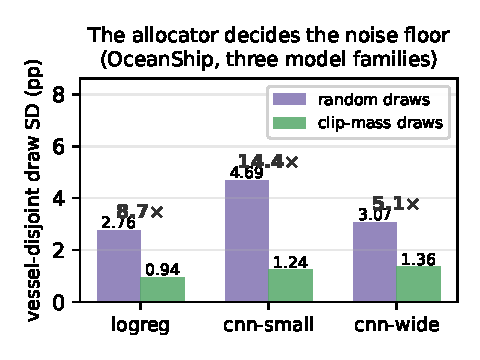
\includegraphics[width=0.46\textwidth]{figures/fig_alloc.pdf}
\hfill
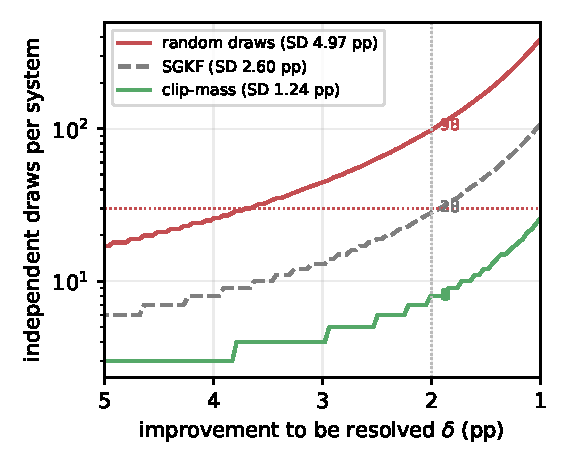
\includegraphics[width=0.5\textwidth]{figures/fig_reqn.pdf}
\caption{Left: Table~\ref{tab:remedy} at a glance---the vessel-disjoint draw SD under random
versus clip-mass allocation, per model family (ratios annotated); the allocator, not the backbone,
decides the observed noise level. Right: independent draws per system required to resolve an improvement of
$\delta$\pp{} ($\alpha=0.05$, power 0.8, two-sample non-central $t$), for the random convention,
\texttt{StratifiedGroupKFold}, and clip-mass allocation; dashed line: a realistic weekly GPU
budget. Planning estimates under SDs measured on 5--25 draws.}
\label{fig:alloc}
\end{figure*}

\subsection{Cross-Model Generalization and Two Instructive Failures}
The collapse holds on every model family tested (Table~\ref{tab:remedy}, Fig.~\ref{fig:alloc}): a
linear probe (variance
ratio $8.7$, exact permutation $p=0.013$), the reference CNN ($14.4$, $p=0.004$), and the wider CNN
($5.1$, $p=0.009$); per-model SD ratios are $0.34$, $0.26$, $0.44$, all under the pre-specified
$0.6$ bar. Two failures sharpen the mechanism. \emph{Count-stratified} allocation, balancing the
number of \emph{vessels} per class, leaves the variance unchanged (ratio $0.93$) with a $+5.4$\pp{}
mean shift (Welch $p=0.096$, not significant---we do not read its direction): vessels carry
3--250 clips each (an
$80\times$ range), so count balance does not balance information mass. \emph{StratifiedGroupKFold}
\cite{sklearn}, the standard tool, halves the variance (ratio $3.25$) but remains $2.4\times$ worse
than clip-mass. In the experiments reported here, stratification had to act on identity-\emph{mass},
not identity counts---and the
composition model predicted both outcomes in advance.

\subsection{A Low-Composition-Variance Control on DeepShip}
\label{sec:control}
The composition model makes a falsifiable cross-corpus prediction. DeepShip's four classes are
balanced and its 609 recordings are numerous relative to the class count, so a random recording-
level draw barely moves the test composition: predicted composition SD $0.30$\pp---an order of
magnitude below OceanShip's $4.3$\pp. Stratification should therefore buy nothing. Consistently,
no variance-reduction benefit is detected under the tested settings
(Table~\ref{tab:control}): random draws $0.699\pm2.95$\pp, clip-mass draws $0.654\pm3.92$\pp, ratio
$1.33$ (inside the pre-specified $[0.6,1.67]$ band; the $-4.5$\pp{} mean shift is not significant,
Welch $p=0.06$---and with 5--6 draws per arm this design cannot establish equivalence, only fail
to detect a benefit). Two further observations strengthen the attribution. First, the frozen splits
reproduce month-earlier values on the same protocol to all reported digits. Second, most of DeepShip's residual draw variance
($\sim$3\pp) is \emph{not} composition (the model explains only $\sim$10\% of it)---it reflects
which individual ships are held out. The predictor is thus discriminative in both directions: it
identifies where the remedy applies (OceanShip, every model family) and where it does not
(DeepShip), before any training run. The ten-draw vessel-disjoint protocol
(Table~\ref{tab:ladder}) completes the picture on both sides: DeepShip's identity leak is real
($0.922 \to 0.624$) even though its composition remedy shows no benefit, and the stricter protocol's
draw variance, now measurable with ten draws, is likewise not composition-shaped ($21.9\%$
explained, permutation $p=0.66$)---the null control holds at the vessel level too. Removing the
leak and stabilizing the remaining variance are two different interventions, and only the second
was ever claimed to be unnecessary on DeepShip. The same ten draws give DeepShip's four-class
structure its honest denominator. Pooled per-class recall under vessel isolation: Tanker
$0.71\pm8$\pp, Passenger $0.66\pm8$\pp, Tug $0.64\pm10$\pp, Cargo $0.52\pm10$\pp---a
$19$\pp{} spread in which every class stays far above the $0.25$ chance rate (pooled macro-F1
$0.61\pm5.4$\pp), against OceanShip's
three-tier collapse under the same protocol (best class $0.75$; nine classes $\le0.07$; four or
five never predicted). Class \emph{granularity}, not corpus identity, decides whether honest
evaluation strands classes: four balanced classes over 609 recordings leave no tail; twelve
AIS-administrative classes over 892 vessels leave nine.

\begin{table}[!t]
\caption{Low-Composition-Variance Control: DeepShip \texttt{rec\_random} (\texttt{cnn\_small}, log-mel)}
\label{tab:control}
\centering
\begin{tabular}{lcccc}
\toprule
Scheme & $n$ & mean & SD (pp) & pred.\ SD (pp) \\
\midrule
random draws (frozen) & 5 & 0.699 & 2.95 & \multirow{2}{*}{0.30} \\
clip-mass draws       & 6 & 0.654 & 3.92 & \\
\bottomrule
\end{tabular}
\end{table}

\section{Limits of Tested Interventions: The Effective Class Structure}
\label{sec:limits}

\subsection{Tested Interventions and Diagnostics}
Under the honest protocol the reference model collapses to three classes (Towing 0.72, Cargo 0.58,
Tug 0.37 recall; nine classes $\le0.07$, four to five never predicted; macro-F1 0.11 against a 0.083
uniform baseline). For every obvious explanation we pre-specified a discriminating experiment and
ran it (Table~\ref{tab:interv}).

\begin{table}[!t]
\caption{Diagnostic Analyses and Tested Interventions for Tail-Class Collapse}
\label{tab:interv}
\centering
\begin{tabular}{p{0.34\columnwidth}p{0.56\columnwidth}}
\toprule
Intervention & Pre-registered test and outcome \\
\midrule
Capacity (ResNet-18, 11.2M) & memorizes the training set (0.9999), tests at 0.378; $+1.0$\pp{}
over \texttt{cnn\_small} \cite{soti2026}. \\
\midrule
Post-hoc prior adjustment & offline logit adjustment on saved probabilities upper-bounds decision-rule
fixes that leave training untouched (it cannot alter learned representations, as in-training loss
re-weighting could): best $+2.0$\pp{} macro-F1 (accuracy $-2.3$\pp). \\
\midrule
Selective prediction & accuracy--coverage curves are flat for three confidence scores
(plots in the release): acc@50\%
$=0.367$ ($+4.9$\pp); a head-only system still answers 97.3\% of tail clips. \\
\midrule
Training-mass analysis & diagnostic dose--response: recall tracks training clip count ($\rho=+0.83$) better than
vessel count ($\rho=+0.68$); 42-vessel Passenger at 0.000 recall. Identity floor confirmed only for
the 2 classes with $<5$ training vessels (pre-specified, hit). \\
\midrule
Frozen pretraining & AudioSet AST \cite{gong2021ast} + linear probe on all 53{,}770 clips: tail
top-2 $0.116$ vs.\ $0.114$ for the small CNN. \\
\midrule
Full fine-tuning & end-to-end AST (2 seeds $\times$ 8 epochs): the only tested remedy that moves
macro-F1 ($0.108\to0.142$), but tail top-2 reaches $0.178$ (GO bar $0.30$); val peaks at epoch 2
then degrades to train-acc 0.81. \\
\bottomrule
\end{tabular}
\end{table}

\subsection{A Three-Tier Tail, Predictable from Metadata}
The fine-tuning gradient is not uniform (Fig.~\ref{fig:tail}): Fishing (top-2
$0.296\to0.442$) and Pleasure Craft ($0.208\to0.339$) are partially rescued; Passenger does not
move; Search-and-Rescue and Tanker stay at zero; head classes are squeezed (Cargo recall
$0.58\to0.32$). Combined with the identity floor (Fig.~\ref{fig:dose}, Table~\ref{tab:dose}) and
the confusion structure
(Fig.~\ref{fig:confusion})---tail classes project 70--80\% of their mass onto Towing, Tanker
projects 60\% onto Tug, Tug itself 37.8\% onto Cargo, and the class means in feature space score
\emph{below} chance---the tail resolves into three tiers: \emph{learnable} (Towing, Cargo, Tug; 3
classes, 61.5\% of clips), \emph{partially rescuable} (Fishing, Pleasure Craft), and
\emph{intervention-resistant} (Passenger, Sailing, SAR, Tanker, and the identity-floor classes Port
Tender, Dredging, and Anti-pollution equipment---a collapse we predicted before running and
confirmed). ``Resistant'' means not recovered by any of the tested interventions; it is not a
claim that no intervention could ever work. The cross-corpus contrast confirms the attribution: the same pipeline learns all four
DeepShip classes under the honest protocol (recalls 0.55--0.75), so the observed contrast is
consistent with a substantial role of the benchmark's label granularity, though it does not
isolate granularity as the sole causal factor; a within-corpus class-merge experiment is the
clean test and remains future work.

\begin{figure}[!t]
\centering
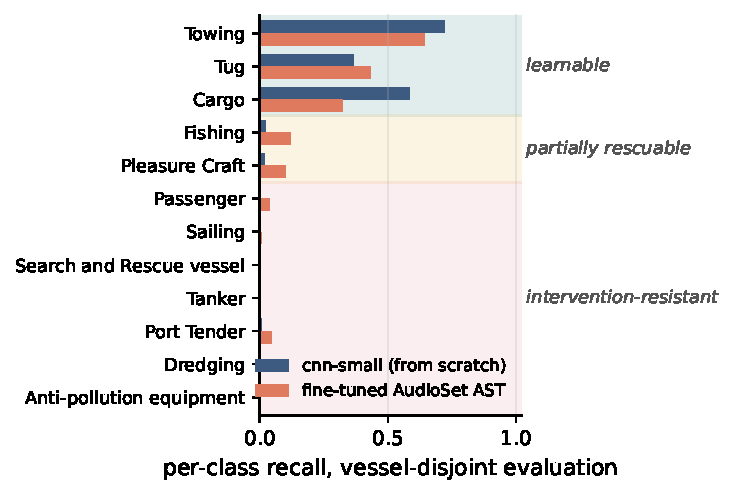
\includegraphics[width=0.78\columnwidth]{figures/fig_tail.pdf}
\caption{Per-class recall under vessel-disjoint evaluation: from-scratch CNN vs.\ fully fine-tuned
AudioSet AST. Shaded tiers: learnable / partially rescuable / intervention-resistant. Fine-tuning
partially rescues the high-mass small-boat classes, leaves Passenger unchanged, cannot revive SAR
and Tanker, and trades away head-class recall.}
\label{fig:tail}
\end{figure}

\begin{figure}[!t]
\centering
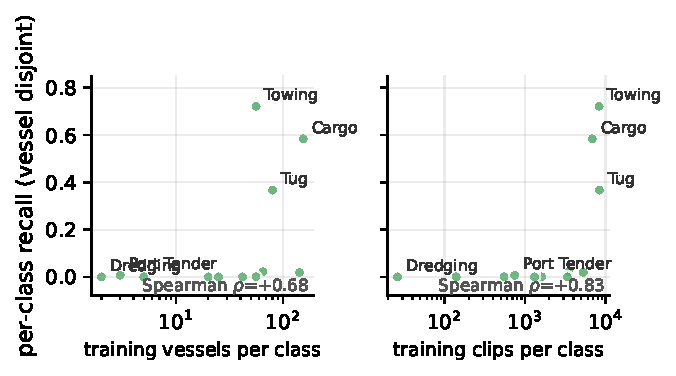
\includegraphics[width=0.8\columnwidth]{figures/fig_dose.pdf}
\caption{Dose--response of per-class recall against training-set identity diversity (log scale).
Recall tracks training \emph{clips} ($\rho=+0.83$) better than training \emph{vessels}
($\rho=+0.68$): identity scarcity floors the two $<5$-vessel classes but is not the main
bottleneck.}
\label{fig:dose}
\end{figure}

\begin{table}[!t]
\caption{Per-Class Metadata and Outcome (vessel-disjoint, pooled 5 draws)}
\label{tab:dose}
\centering
\begin{tabular}{lccc}
\toprule
Class & recall & train vessels & train clips \\
\midrule
Towing                 & 0.722 & 56  & 8{,}306 \\
Cargo                  & 0.584 & 155 & 6{,}837 \\
Tug                    & 0.367 & 80  & 8{,}382 \\
Fishing                & 0.022 & 65  & 3{,}510 \\
Pleasure Craft         & 0.019 & 143 & 5{,}287 \\
Port Tender            & 0.007 & 3   & 743 \\
Passenger              & 0.000 & 42  & 3{,}346 \\
Sailing                & 0.000 & 46  & 1{,}099 \\
Search and Rescue      & 0.000 & 15  & 318 \\
Tanker                 & 0.000 & 13  & 112 \\
Anti-pollution         & 0.000 & 5   & 18 \\
Dredging               & 0.000 & 2   & 26 \\
\bottomrule
\multicolumn{4}{l}{\footnotesize Passenger (42 vessels, 3{,}346 clips) refutes vessel}\\
\multicolumn{4}{l}{\footnotesize count as the bottleneck; Port Tender and Dredging}\\
\multicolumn{4}{l}{\footnotesize confirm the pre-specified identity floor.}
\end{tabular}
\end{table}

\begin{figure}[!t]
\centering
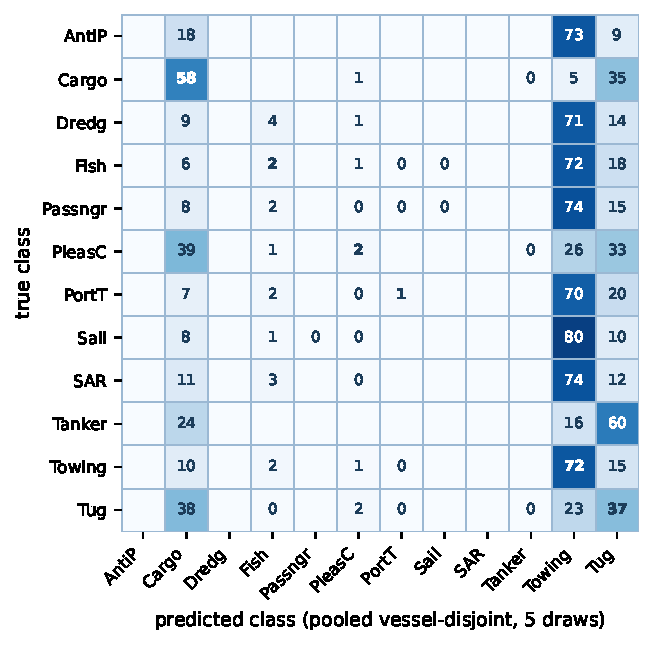
\includegraphics[width=0.85\columnwidth]{figures/fig_confusion.pdf}
\caption{Row-normalized confusion matrix (pooled over five vessel-disjoint draws). Tail-class mass
flows almost exclusively into the three head columns; within the tail, confusion is diffuse. Under
the honest protocol the 12-class benchmark behaves as a 3-class problem.}
\label{fig:confusion}
\end{figure}

\section{A Reporting Recipe}
The audit reduces to five reportable numbers, all computable without new modelling:
(1) the allocation unit, and how the corpus slices recordings into clips (tiling ratio, clips per
recording, stream-position availability);
(2) the number of independent draws and the draw-to-draw SD per scheme;
(3) the composition share of that SD via Eq.~\eqref{eq:comp};
(4) the required-$N$ table for the claimed effect size (Fig.~\ref{fig:alloc} (right));
(5) the effective class structure under the honest protocol (per-class recall and top-2,
never-predicted classes, $<5$-identity floors).
We release the frozen splits, the allocator, and the required-$N$ calculator so that this is a
five-minute post-processing step rather than a re-review.

\section{Discussion and Limitations}
\subsection{Relation to Existing Guidance}
Published guidance says \emph{what} to do (use recording- or identity-level
splits) and \emph{why} (adjacent clips share noise and propagation conditions \cite{review2026});
it does not say what the change does to the statistics of an evaluation. Our numbers supply the
missing half: the honest protocol multiplies draw noise by $12\times$, that noise is $89\%$
composition (59\% predictable out-of-sample) and therefore largely foreseeable before training,
and the remedy makes rigorous comparison
affordable ($\sim$100$\to$8 unpaired draws per system; measured on real model pairs, pairing alone
cuts the requirement to 10--13 under the non-central-$t$ power calculation---the paired-difference
SD is $1.9$--$2.3$\pp, not the $5.6$\pp{} independence would predict---and adding the allocator
cuts it again to 3--7). We also learned the aggregation lesson the hard way: an unfiltered
pool of 25 vessel-disjoint runs of mixed provenance---six allocation schemes and two probes, a
superset of and distinct from the 25 random draws of Table~\ref{tab:ladder}---has a
draw-to-draw SD of $8.2$\pp, which pools between-scheme variance with draw variance. Re-aggregated
per scheme (released scripts), the same runs reproduce $5.0$\pp{} under the random allocator and
$1.2$\pp{} under clip-mass: tag-aware aggregation is not optional bookkeeping but the difference
between a statistic and a mixture. This reframes identity-disjoint evaluation from ``a stricter
convention'' into ``a protocol with known, managed statistics''---the same transition clinical
research underwent when multi-centre variance moved from anecdote to design parameter.

\subsection{What the Remedy Does and Does Not Claim}
Clip-mass allocation does not make models better;
it makes comparisons cheaper and honest numbers stable. The $4.69\to1.24$\pp{} collapse means a
two-draw comparison that would have been dominated by composition noise becomes meaningful, and
paired designs (same draws for all systems) compose with it for a further
measured $3$--$4\times$ reduction in the number of draws (Sec.~\ref{sec:remedy}). The remedy also removes the composition
\emph{bias} of random draws: a random vessel draw can make the test set systematically easier or
harder than the corpus, and averaging over few draws does not fix a biased draw.

\subsection{Threats to Validity}
\label{sec:threats}
\emph{Internal.} All comparisons share one frozen split family and one recipe; run identifiers
encode recipe and protocol, and every run's final learning rate is logged and checked. The recall
table feeding the predictor was frozen before the scored schemes' draws existed
(Sec.~\ref{sec:predictor}). \emph{External.} The remedy is validated on one corpus's honest protocol across three
model families, with the null control on a second; a third corpus with intermediate composition
variance would complete the dose--response. Both benchmarks also ultimately draw on recordings
from the same regional collection network (Ocean Networks Canada, Strait of Georgia)---on disjoint vessels, recording campaigns, and periods---so the null control demonstrates that the
composition \emph{mechanism} generalizes across corpora, not that the recording conditions are
independent; a corpus collected outside this network remains the missing external point.
Absolute accuracies are low ($0.24$--$0.37$); our
claims concern \emph{variance and structure}, which we argue are protocol properties, and the
capacity/pretraining interventions bound the role of model choice. A SOTA-scale system would shift
the per-class recall table feeding the predictor---but the predictor is re-estimated per system
from its own random draws, so the framework, not the constants, is the contribution.
\emph{Construct.} Equation~\eqref{eq:comp} holds the per-class recalls fixed: it cannot capture
draw-specific recall variation arising from training-ship identity, test-ship difficulty, or
acoustic conditions; class interactions, if present, are one possible contributor among these.
The DeepShip residual (composition explains only $\sim$10\% of a
still-substantial 3\pp{} spread) makes this visible. The 85\% share of the pre-specified five-draw
analysis was re-estimated independently on the released 25-draw pool (89.0\%, permutation
$p=0.0006$; Table~\ref{tab:decomp}); the remedy pools ($n{=}6$ per scheme) and the DeepShip
vessel pool ($n{=}10$: $21.9\%$, $p=0.66$, consistent with the null control) remain too small for
their own decomposition---the required-$N$ analysis of Sec.~\ref{sec:variance} applies to our own
confirmatory pipeline as much as to anyone's. Fine-tuned AST ran with two seeds at a fixed
budget; the tail conclusion rests on the pre-specified bar rather than an exhaustive sweep.
\emph{Labels.} OceanShip's AIS categories are administrative fishing-vessel, port-tug,
rescue-boat classes, not acoustic families. Our results quantify that mismatch---the effective
class structure has three tiers, and the metadata predicts which classes
fall in which---but do not claim it is universal. Benchmarks built from operational metadata
should expect exactly this analysis.

\section{Conclusion}
Honest evaluation in UATR is currently a trade with unquantified terms: identity-disjoint splits
remove a real leak and, on OceanShip, replace $0.4$\pp{} of clip-level noise with $5.0$\pp{} of
metadata-driven noise that single-draw papers silently absorb. We showed this noise is 89\%
composition (59\% predictable out-of-sample), removable by a class-mass allocation to the lowest
variability observed across the tested allocations
($14.4\times$ variance reduction, exact permutation $p=0.004$), general across model families, and correctly
predicted to be unnecessary on DeepShip. We also showed what the resulting honest numbers mean: a
three-tier effective class structure that the tested interventions---including full fine-tuning of an
AudioSet-pretrained transformer---cannot open beyond its predicted limits under the tested
settings. Benchmarks should report
the allocation scheme, the draw variance, and the effective class structure; without them,
``accuracy on OceanShip'' is not one number but a distribution.

\section*{Acknowledgments}
The authors thank the OceanShip, DeepShip, and ShipsEar teams for their data and metadata, Ocean
Networks Canada for hydrophone access, and Kaggle for compute.

\section*{Reproducibility}
Frozen splits (SHA-256-seeded, content-verified at load), all training and evaluation code, the
allocation scripts, per-clip predictions for every run, the required-$N$ calculator, a run
manifest (\texttt{run\_manifest.csv}: one row per released draw with corpus, model, protocol,
allocation scheme, split seed, and metrics), and the machine-readable aggregation outputs
(\texttt{w3e\_bootstrap.json}, \texttt{w3e2\_variance.json}, \texttt{w3e3\_lodo.json}) are
released at \url{https://github.com/gzhgzy1234567890-lang/uatr-honest-evaluation} (a DOI-minted
archive follows at acceptance). Every table
regenerates from the released per-draw
files. On DeepShip, the 48 recordings whose AIS join failed enter the vessel-disjoint protocol as
singleton vessels (group key \texttt{singleton::<rec\_key>}); the runner's leak check applies the
same rule, so what the split promises and what it verifies are identical.

{\footnotesize
\begin{thebibliography}{99}

\bibitem{review2026}
C.~Yan, R.~Gao, G.~Pan, Y.~Yu, S.~Yan, J.~Xu, Y.~Yang, T.~Yao, and J.~Li, ``Review of underwater
acoustic target recognition technology: From machine learning to deep learning'' (in Chinese),
\emph{Digital Ocean \& Underwater Warfare}, vol.~9, no.~2, pp. 118--130, 2026,
doi:10.19838/j.issn.2096-5753.2026.02.001.

\bibitem{uniqueship2026}
C.~Hashemi, T.~Stout, A.~Hoogs, and J.~Parham, ``UniqueShip: Mitigating data leakage in acoustic
ship classification benchmark datasets,'' arXiv:2609.13659, 2026 (accepted, OCEANS 2026).

\bibitem{boosting2026}
C.~Yan, S.~Yan, Y.~Yu, R.~Gao, G.~Pan, Y.~Yang, T.~Yao, and P.~N.~Suganthan,
``Boosting-inspired sequential multi-head learning for underwater acoustic target recognition,''
\emph{Ocean Engineering}, vol.~356, art. 125324, 2026, doi:10.1016/j.oceaneng.2026.125324.

\bibitem{kapoor2023}
S.~Kapoor and A.~Narayanan, ``Leakage and the reproducibility crisis in machine-learning-based
science,'' \emph{Patterns}, vol.~4, no.~9, 2023.

\bibitem{bouthillier2021}
X.~Bouthillier \emph{et al.}, ``Accounting for variance in machine learning benchmarks,'' in
\emph{Proc.\ MLSys}, 2021 (arXiv:2103.03098).

\bibitem{mpds2026}
K.~Shao, ``Metadata predictability is not evidence dependence: An intervention-based audit for
weak-label benchmarks,'' arXiv:2605.23701, 2026 (ICML 2026 Workshop on Hypothesis Testing).

\bibitem{gillick1989}
L.~Gillick and S.~J.~Cox, ``Some statistical issues in the comparison of speech recognition
algorithms,'' in \emph{Proc.\ IEEE Int.\ Conf.\ Acoustics, Speech, and Signal Processing
(ICASSP)}, Glasgow, U.K., 1989, pp. 532--535, doi:10.1109/ICASSP.1989.266481.

\bibitem{sklearn}
F.~Pedregosa \emph{et al.}, ``Scikit-learn: Machine learning in Python,'' \emph{JMLR}, vol.~12,
2011. (StratifiedGroupKFold: scikit-learn $\ge$1.0.)

\bibitem{deepship}
M.~Irfan, Z.~Jiangbin, S.~Ali, M.~Iqbal, Z.~Masood, and U.~Hamid, ``DeepShip: An underwater
acoustic benchmark dataset and a separable convolution based autoencoder for classification,''
\emph{Expert Systems with Applications}, vol.~183, art. 115270, 2021,
doi:10.1016/j.eswa.2021.115270.

\bibitem{shipsear}
D.~Santos-Dom\'inguez, S.~Torres-Guijarro, A.~Cardenal-L\'opez, and A.~Pena-Gim\'enez,
``ShipsEar: An underwater vessel noise database,'' \emph{Applied Acoustics}, vol.~113,
pp. 64--69, 2016.

\bibitem{oceanship}
Z.~Li, S.~Xiang, T.~Yu, J.~Gao, J.~Ruan, Y.~Hu, T.~Liu, and Y.~Fu, ``OceanShip: A large-scale
dataset for underwater audio target recognition,'' in \emph{Proc.\ ICIC}, LNCS, 2024
(arXiv:2401.02099).

\bibitem{hummel2026}
H.~I.~Hummel, S.~Bhulai, R.~van~der~Mei, and B.~Ghani, ``Linear probing enables ship-radiated
noise recognition with pretrained audio embeddings,'' \emph{Ecological Informatics}, vol.~95,
art. 103709, 2026, doi:10.1016/j.ecoinf.2026.103709 (arXiv:2601.08358).

\bibitem{aa2025contrastive}
H.~Hummel, A.~Gansekoele, S.~Bhulai, and R.~van~der~Mei, ``The computation of generalized
embeddings for underwater acoustic target recognition using contrastive learning,''
\emph{Applied Acoustics}, vol.~243, art. 111103, 2026, doi:10.1016/j.apacoust.2025.111103.

\bibitem{fang2025}
H.~Fang, Y.~Xie, J.~Ren, W.~Wang, and J.~Xu, ``A momentum-based adversarial training approach
for generalization in underwater acoustic target recognition: An individual-vessel
perspective,'' \emph{Journal of the Acoustical Society of America}, vol.~157, no.~5,
pp. 3508--3523, 2025, doi:10.1121/10.0036456.

\bibitem{mmipfnn2026}
F.~Liu, Z.~Li, K.~Yang, F.~Chen, and J.~Yu, ``MmPiFNN: A multi-mode physics-informed fuzzy neural
network for passive recognition of surface ships by underwater equipment using ship radiated noise
signals,'' \emph{Defence Technology}, vol.~59, pp. 243--266, 2026, doi:10.1016/j.dt.2025.11.003.

\bibitem{soti2026}
A.~Soti, T.~P.~Sone, N.~Ibnul, H.~H.~Aung, H.~Zhong, G.~Cohen, and Y.~Xu, ``Towards deployable
underwater vessel classification,'' arXiv:2609.29179, 2026.

\bibitem{gong2021ast}
Y.~Gong, Y.-A. Chung, and J.~Glass, ``AST: Audio spectrogram transformer,'' in \emph{Interspeech},
2021.
\end{thebibliography}
}\end{document}
